\documentclass[solutionbox,answers]{exam}

%%%%%%%%%%%%%%%%%%%%%%%%%%%%%%%%%%%%%%%%%%%%%%%%%%%%%%%%%%%%%%%
% Update to change header
\newcommand{\courseName}{CS 577}
\newcommand{\assignmentName}{Assignment 8 -- Dynamic Programming 2}
\newcommand{\semester}{Spring 2023}
%%%%%%%%%%%%%%%%%%%%%%%%%%%%%%%%%%%%%%%%%%%%%%%%%%%%%%%%%%%%%%%

\usepackage[utf8]{inputenc}
\usepackage[T1]{fontenc}

\usepackage{amsmath}
\usepackage{amsfonts}
\usepackage{amsthm}
\usepackage{booktabs}
\usepackage[ruled]{algorithm2e}
\usepackage{graphicx}
\usepackage[rightcaption]{sidecap}  % for positioning figure captions to the left or right of the figure

\usepackage{hyperref}

\pagestyle{headandfoot}
\runningheadrule
\firstpageheader{\courseName}{\huge \assignmentName}{\semester}
\runningheader{\courseName}
{\assignmentName}
{\semester}
\firstpagefooter{}{}{}
\runningfooter{}{Page \thepage\ of \numpages}{}

\sidecaptionvpos{figure}{c}
\renewcommand\sidecaptionsep{1cm}

\begin{document}

\begin{center}
\setlength{\fboxsep}{10pt}
\fbox{\parbox{5.5in}{
Answer the questions in the boxes provided on the
question sheets. If you run out of room for an answer,
add a page to the end of the document. 
}}
\end{center}
\vspace{0.1in}
\makebox[0.47\textwidth]{Name:\enspace\hrulefill} \qquad
\makebox[0.47\textwidth]{Wisc id:\enspace\hrulefill}

\section*{Dynamic Programming}

Do \textbf{NOT} write pseudocode when describing your dynamic programs. Rather give the Bellman Equation, describe the matrix, its axis and how to derive the desired solution from it.

%%%%%%%%%
\begin{questions}

\question \textit{Kleinberg, Jon. Algorithm Design (p. 327, q. 16).} 

In a hierarchical organization, each person (except the ranking officer) reports to a unique superior officer. The reporting hierarchy can be described by a tree $T$, rooted at the ranking officer, in which each other node $v$ has a parent node $u$ equal to his or her superior officer. Conversely, we will call $v$ a direct subordinate of $u$. 

Consider the following method of spreading news through the organization. 
\begin{itemize}
\item The ranking officer first calls each of her direct subordinates, one at a time. 
\item As soon as each subordinate gets the phone call, he or she must notify each of his or her direct subordinates, one at a time. 
\item The process continues this way until everyone has been notified. 
\end{itemize}

Note that each person in this process can only call \textit{direct} subordinates on the phone. 

We can picture this process as being divided into rounds. In one round, each person who has already heard the news can call one of his or her direct subordinates on the phone. The number of rounds it takes for everyone to be notified depends on the sequence in which each person calls their direct subordinates.

\begin{SCfigure}[50][h]
    % \centering
    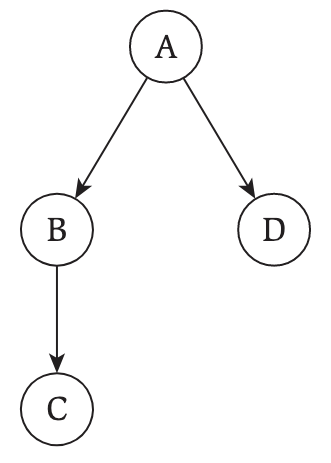
\includegraphics[width=0.15\textwidth]{figures/q3.png}
    \caption{A hierarchy with four people. The fastest broadcast scheme is for A to call B in the first round. In the second round, A calls D and B calls C. If A were to call D first, then C could not learn the news until the third round.}
    \label{fig:q3}
\end{SCfigure}

The questions are on the next page. 
\newpage

Give an efficient algorithm that determines the minimum number of rounds needed for everyone to be notified, and outputs a sequence of phone calls that achieves this minimum number of rounds by answering the following: 
\begin{parts}
\item Give a recursive algorithm. (The algorithm does not need to be efficient)
\begin{solutionbox}{\stretch 1} \vspace{1em} 

\end{solutionbox}

\item Give an efficient dynamic programming algorithm.
\begin{solutionbox}{\stretch 1} \vspace{1em} 

\end{solutionbox}

\item Prove that the algorithm in part (b) is correct.
\begin{solutionbox}{\stretch 1} \vspace{1em} 

\end{solutionbox}
\end{parts}

\newpage

%%%%%%%%%

\question 
Consider the following problem: you are provided with a two dimensional matrix $M$ (dimensions, say, $m \times n$). 
Each entry of the matrix is either a \textbf{1} or a \textbf{0}. 
You are tasked with finding the total number of square sub-matrices of $M$ with all \textbf{1}s. 
Give an $O(mn)$ algorithm to arrive at this total count by answering the following:

\begin{parts}
  \item Give a recursive algorithm. (The algorithm does not need to be efficient)
  \begin{solutionbox}{\stretch 1} \vspace{1em} 
  
  \end{solutionbox}
  
  \item Give an efficient dynamic programming algorithm.
  \begin{solutionbox}{\stretch 1} \vspace{1em} 
  
  \end{solutionbox}
  
  \item Prove that the algorithm in part (b) is correct.
  \begin{solutionbox}{\stretch 1} \vspace{1em} 
  
  \end{solutionbox}

  \item Furthermore, how would you count the total number of square sub-matrices of $M$ with all \textbf{0}s?
  \begin{solutionbox}{\stretch 1} \vspace{1em} 
  
  \end{solutionbox}
  \end{parts}
\newpage

%%%%%%%%


\question \textit{Kleinberg, Jon. Algorithm Design (p. 329, q. 19).} 

String $x'$ is a \emph{repetition} of $x$ if it is a prefix of $x^k$ ($k$ copies of $x$ concatenated
together) for some integer $k$. So $x' = 10110110110$ is a repetition of $x = 101$.
We say that a string $s$ is an \textit{interleaving} of $x$ and $y$ if its symbols can be partitioned into two (not necessarily contiguous) subsequences $x'$ and $y'$, so that $x'$ is a repetition of $x$ and $y'$ is a repetition of $y$. 
For example, if $x = 101$ and $y = 00$,
then $s = 100010010$ is an interleaving of $x$ and $y$, since characters $1,2,5,8,9$ form $10110$—a repetition of $x$—and the remaining characters $3,4,6,7$ form
$0000$—a repetition of $y$.

Give an efficient algorithm that takes strings $s$, $x$, and $y$ and decides if $s$ is an interleaving of $x$ and $y$ by answering the following:

\begin{parts}
  \item Give a recursive algorithm. (The algorithm does not need to be efficient)
  \begin{solutionbox}{\stretch 1} \vspace{1em} 
  
  \end{solutionbox}
  
  \item Give an efficient dynamic programming algorithm.
  \begin{solutionbox}{\stretch 1} \vspace{1em} 
  
  \end{solutionbox}
  
  \item Prove that the algorithm in part (b) is correct.
  \begin{solutionbox}{\stretch 1} \vspace{1em} 
  
  \end{solutionbox}
  \end{parts}

\newpage

%%%%%%%%%

\question \textit{Kleinberg, Jon. Algorithm Design (p. 330, q. 22).} 

To assess how “well-connected” two nodes in a directed graph are, one can not only look at the length of the shortest path between them, but can also count the number of shortest paths. 

This turns out to be a problem that can be solved efficiently, subject to some restrictions on the edge costs. Suppose we are given a directed graph $G = (V, E)$, with costs on the edges; the costs may be positive or negative, but every cycle in the graph has strictly positive cost. We are also given two nodes $v, w\in V$. 

Give an efficient algorithm that computes the number of shortest $v-w$ paths in $G$. (The algorithm should not list all the paths; just the number suffices.) 

  \begin{solutionbox}{\stretch 1} \vspace{1em} 

  \end{solutionbox}

\newpage

%%%%%%%%%

\question The following is an instance of the Knapsack Problem. 
Before implementing the algorithm, run through the algorithm by hand on this instance. 
To answer this question, generate the table, indicate the maximum value, and recreate the subset of items.

\begin{center}
\begin{tabular}{ |c|c|c| } 
 \hline
 item & weight & value \\ 
\hline
\hline
 1 & 4 & 5 \\ 
\hline
 2 & 3 & 3 \\ 
\hline
 3 & 1 & 12 \\ 
\hline
 4 & 2 & 4 \\ 
 \hline
\end{tabular}

Capacity: 6
\end{center}
  \begin{solutionbox}{\stretch 1} \vspace{1em} 

  
  \end{solutionbox}

%%%%%%%%%

\question Implement the algorithm for the Knapsack Problem in either C, C++, C\#, Java, or Python. Be efficient and implement it in $O(nW)$ time, where $n$ is the number of items and $W$ is the capacity.

The input will start with an positive integer, giving the number of instances that follow. For each
instance, there will two positive integers, representing the number of items and the capacity, followed by a list describing the items.
For each item, there will be two nonnegative integers, representing the weight and value, respectively.

A sample input is the following:

\begin{verbatim}
2
1 3
4 100
3 4
1 2
3 3
2 4
\end{verbatim}
The sample input has two instances. The first instance has one item and a capacity of 3. The item has weight 4 and value 100. 
The second instance has three items and a capacity of 4.

For each instance, your program should output the maximum possible value.
The correct output to the sample input would be:

\begin{verbatim}
0 
6
\end{verbatim}

\end{questions}

\end{document}
